%\documentstyle[moreverb,code,wrapfig,11pt]{article}
\documentclass[11pt]{article}
\usepackage{epsfig,fancyvrb}
\usepackage{wrapfig,code,moreverb}
\setlength{\topmargin}{-0.4in}
\setlength{\oddsidemargin}{+0.0in}
\setlength{\evensidemargin}{+0.0in}
\setlength{\textheight}{8.5in}
\setlength{\textwidth}{6.50in}
\setlength{\marginparwidth}{0.0in}
\setlength{\marginparsep}{0.0in}
\setlength{\marginparpush}{0.0in}
\setlength{\unitlength}{1.0in}
\setlength{\parskip}{.1in}
\renewcommand{\bottomfraction}{.90}
\renewcommand{\topfraction}{.90}
\makeatletter
\date{}
\def\tightitemize{\ifnum \@itemdepth >3 \@toodeep\else \advance\@itemdepth \@ne
\edef\@itemitem{labelitem\romannumeral\the\@itemdepth}%
\list{\csname\@itemitem\endcsname}{\setlength{\topsep}{-\parskip}\setlength{\parsep}{0in}\setlength{\itemsep}{0in}\setlength{\parskip}{0in}\def\makelabel##1{\hss\llap{##1}}}\fi}
 
\let\endtightitemize =\endlist
\begingroup
 \catcode`\`=\active
 \gdef\verbatim@font{\footnotesize\tt \catcode96\active
   \def`{\leavevmode\kern\z@\char96 }}
\endgroup
\makeatother
\newcommand{\longpage}{\enlargethispage{\baselineskip}}
\newcommand{\shortpage}{\enlargethispage{-\baselineskip}}
\pssilent
\pagestyle{empty}
\renewcommand{\baselinestretch}{.95}   % -- double spaced lines
\title{The Connection Manager Library}
\author{ 
\large\bf Greg Eisenhauer\\
eisen@cc.gatech.edu\\
\ \\
College of Computing \\
Georgia Institute of Technology \\
Atlanta, Georgia 30332 \\
}
\begin{document}
\bibliographystyle{plain}
% \begin{titlepage}
\maketitle
\begin{center}
\today{} -- CM/EVPath Version 3.0
\end{center}
\section{Introduction}

Connection Manager is a library of communications routines which manage the
complexity of systems with multiple communication links between
heterogeneous machines.  The library is designed to be used as an
implementation basis for networks of agents communicating
application-specific data.  It contains support for establishing communication between agents,
matching incoming messages with handlers, and assisting in the distribution
of message format information to entities with which it is communicating.
Connection Manager is a point-to-point messaging API contained within
the broader EVPath library.  This paper details the services and
interfaces offered by CM.

\section{Overall Description\label{overall}}

The core purpose of Connection Manager is to ease the task of creating and
operating networks of communicating entities over specialized and
configurable data transport mechanisms.  In particular, it is designed to
abstract away the intricacies of those transports and to satisfy two
conflicting goals: allowing uncustomized applications and libraries to
transparently use specialized data transport mechanisms (such as raw
ATM, InfiniBand, Reliable UDP), while still allowing knowledgeable
application layers to configure transport particulars.

CM also directly supports heterogeneous applications by providing for binary
data transmission between entities and locating the most appropriate handler
for incoming data.  To provide heterogeneity support, CM relies mostly
upon FFS, a lower-level communications library that supports binary
transmission of C-style data structures between heterogeneous machines.
FFS is documented in the {\bf FFS Reference Manual}, available at
http://www.cc.gatech.edu/\~{ }eisen/FFS\_manual.pdf.  That document is not
yet complete.  It began it's life as a manual for PBIO, FFS'
predecessor, and has not yet been completely updated.
Familiarity with the concepts
and specifications used in FFS are necessary for understanding messaging in
CM.  Under normal circumstance, CM relies on FFS's internal mechanisms for
distributing message format information.  However, in circumstances where
dependency upon FFS's external format server is impossible, such as for
operation within the kernel, each CM application can act as its own format
server.

\begin{figure}
\vspace*{-0.35in}
\begin{center}\
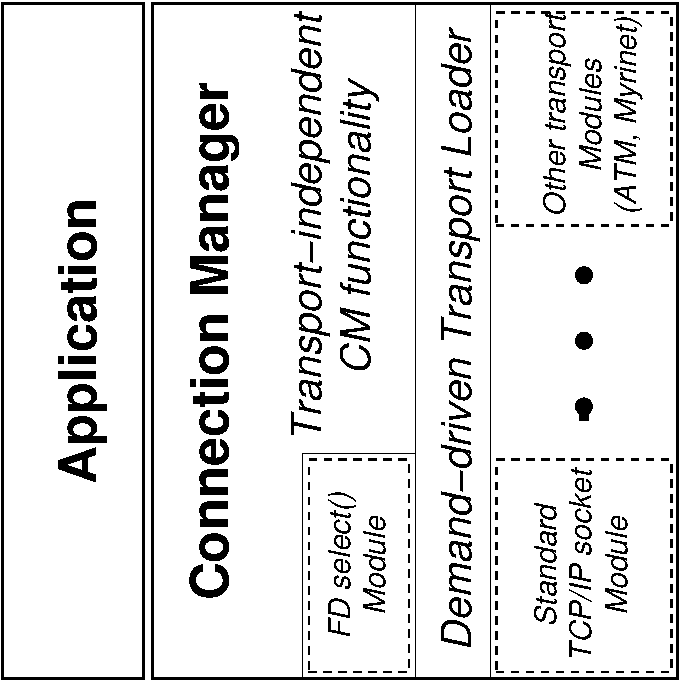
\includegraphics[angle=270,width=3in]{struct.pdf}
%\psfig{figure=struct.eps,width=3in}
\caption{Structure of the Connection Manager.\label{fig:struct}} 
\end{center}
\end{figure}
In order to allow applications to transparently use a variety of data
transport mechanisms, CM is structured so that individual transports are
implemented with dynamically loadable modules as depicted in
Figure~\ref{fig:struct}.  Applications can use transport mechanisms that
might not have existed when the application as written and they are not
burdened with the code and memory requirements of unused transports.  In
addition to the dynamically loadable transports, Figure~\ref{fig:struct}
shows {\it FD select()} functionality separated out into a loadable module.
This module provides control-flow support for transports which may be
integrated into the OS file descriptor system.  Its separation into a
loadable module allows CM to be used as a communications manager even in
situations where {\it FD select()} is not a viable control-flow mechanism,
such as within the OS kernel.

In addition to allowing applications to transparently use different data
transport mechanisms, CM is also designed to allow more aware applications
to customize the behavior of those data transports, for example to specify
bandwidth requirements, expected reliability or other transport-specific
characteristics.  Because CM does not have {\it a priori} knowledge of the
specific transports that might be used by an application, it must have a
mechanism though which it can pass virtually any type of parametric
specification between applications and the selected data transport.  This
role is filled by {\it attribute lists}.  An attribute is a {\it name/value}
pair that specifies something about a connection or message.  Lists of these
attributes are used to specify to CM the characteristics of the connections
it should make.  For example, a standard TCP/IP connection might be
specified by the attribute list:  
\begin{verbatim}
{IP_HOST,"latte.cc.gatech.edu"},{IP_PORT,40767}
\end{verbatim}
Attribute lists are used by CM for a variety of other purposes as well, in
both the application-layer API and in communication with the data transport
modules.   
\enlargethispage{\baselineskip}
\pagebreak

\begin{wrapfigure}[31]{r}{3.7in}
{
\vspace*{-0.35in}
\begin{verbatim}
#include <stdio.h>
#include "atl.h"
#include "evpath.h"

typedef struct _msg {
    char *string_field;
} msg, *msg_ptr;

static FMField msg_field_list[] =
{
    {"string_field", "string", sizeof(char*), 0},
    {NULL, NULL, 0, 0}
};


static void
msg_handler(CManager cm, CMConnection conn, void *msg,
        void *client_data, attr_list attrs)
{
    printf("%s\n", ((msg_ptr)msg)->string_field);
}

int
main (int argc, char **argv)
{
    CManager cm;
    CMFormat format;
    attr_list contact_list;

    cm = CManager_create();
    CMlisten(cm);
    contact_list = CMget_contact_list(cm);
    printf("Contact list \"%s\"\n", 
           attr_list_to_string(contact_list));
    format = CMregister_simple_format(cm, "hello", 
                                      msg_field_list, sizeof(msg));
    CMregister_handler(format, msg_handler, NULL);
    CMrun_network(cm);
}
\end{verbatim}
}
\end{wrapfigure}
\subsection{A ``Hello, World!'' Program\label{hello}}
At this point it is useful to discuss Connection Manager in the context of a
simple program.  The program at the right is the receiving side of a basic
``Hello, World!'' program.  CM provides a
reactive programming style.  That is, most programs are structured around
the exchange of messages, utilizing CM's ability to call
application-specified handlers when messages of appropriate types arrive.
This particular program does nothing except wait for the arrival of a
``hello'' message.  When one arrives, the subroutine \verb+msg_handler()+ is
called and it prints out the \verb+string_field+ element of the message.

The \verb+typedef+ at the beginning of the program declares the datatype of
the message.  The \verb+FMField+ declaration creates a FFS-style
\verb+FMFieldList+ that is used to describe the message datatype to the
Connection Manager.  The subroutine \verb+msg_handler()+ has a prototype
shared by all CM message handlers.  It has parameters representing the
calling Connection Manager, the connection on which the message was
received, a pointer to the message data (as a \verb+void*+ pointer, and
the \verb+client_data+ parameter that was given by the application when the
handler was registered.

This program uses five basic CM functions:
\begin{description}
\item[{\tt CManager\_create()}] --  This call creates and initializes a {\tt
CManager} 
data structure.  All CM applications must call this at least once.
The {\tt CManager} data structure provides a means of associating related
communication channels.   Essentially, the CManager is a {\tt control
context} in which network messages are handled.
\item[{\tt CMlisten(CManager cm)}] -- This call requests CM to listen for
incoming network connections.  What exactly this does depends upon what
network transport layer is in use.  In the default ``sockets'' transport,
this will cause CM to create an internet socket on the current host, bind it
to randomly chosen IP port {\tt port\_num} and begin listening for
connections.  Once {\tt CMlisten()} has been called, other programs can
initiate a connection with this program by calling {\tt CMinitiate\_conn()}
discussed further below.   The contact information for a CM is encapsulated
in an {\it attribute list}.  {\it The contents of the attribute list are
transport-specific.  Casual CM users should consider these attribute lists
to be opaque.}  However, the goal of CM is that these attribute lists might
provide the mechanism through which application-specific transport
requirements, such as QOS specifications, can be communicated to the
transport layer.  Applications with detailed knowledge of the transport in
use can use:
\begin{verbatimtab}
	extern int CMlisten_specific (CManager cm, attr_list listen_info);
\end{verbatimtab}
to pass specific attributes to the transport-based listen call.  In
particular, the ``sockets'' transport looks for an ``IP\_PORT'' attribute to
specify the port upon which it is to listen.

\newsavebox{\mybox}
\sbox{\mybox}{\makebox[6.4in][l]{\parbox{6.457in}{\tt CMFormat CMregister\_simple\_format(CManager cm, char
*format\_name,\\ \hspace*{2.63in}FMFieldList field\_list, int struct\_size);}}}
\item[{\usebox{\mybox}}]\ \\
{\bf --} This routine provides the basic mechanism for making message
formats known to CM.  Registration is a prerequisite for handler
registration or writing data of that format.  The {\tt field\_list}
parameter is a FFS field list specifying the structure of the message.
Record format descriptors are described in the FFS documentation, but
basically consist of a list of field descriptions, where  each field
description is a quadruple giving the field name, data type, size and offset
within the record.  Given this information (along with the format name
and the overall size of the structure)\footnote{Because of structure
  alignment considerations in the compiler, structure size cannot
  always be accurately inferred from information such as the size and
  offset of the last field.  Therefore is should be specified
  explicitly with a 'sizeof()' argument as shown in the examples.}, FFS can pack the record for
transmission to other machines and can decode it despite differences in
machine architecture or record layout.  

CMregister\_simple\_format() can only be used to register message
types that do not have internal substructures.  For more complex data
types, one should use 
\newsavebox{\minebox}
\sbox{\minebox}{\makebox[6.4in][l]{\parbox{6.457in}{\tt CMFormat
      CMregister\_format(CManager cm, FMStructDescList format\_list);}}}
\item[{\usebox{\minebox}}].  The {\tt format\_list} parameter is a list of
format\_name/field\_list pairs as below:
\begin{verbatimtab}
	typedef struct _FMformat_list {
	    char *format_name;
	    FMFieldList field_list;
	    int struct_size;
	    FMOptInfo *opt_info;
	} FMStructDescRec, *FMStructDescList;
\end{verbatimtab}
and is used to specify the representation of the top-level structure
(entry 0 in the list) and any nested structures in the
message.  It should contain the transitive closure of all data types
necessary to specify the message representation.  The list is
terminated with a \verb+{NULL, NULL, 0, NULL}+ value. 

\item[\parbox{6.4in}{\tt void CMregister\_handler(CMFormat format, CMHandlerFunc handler,\\
\hspace*{1.9in}void *client\_data)}] \ \\
-- {\tt CMregister\_handler()} binds the
subroutine specified in its {\tt handler} parameter to the arrival of
messages of the type {\tt format}.  The profile of the handler function
should be:
\begin{verbatimtab}
typedef void (*CMHandlerFunc) (CManager cm, CMConnection conn,
                               void *message, void *client_data, attr_list attrs);
\end{verbatimtab}
The {\tt client\_data} parameter specified in the registration call is not
interpreted by CM, but merely passed to the handler function when it is
called.   
The {\tt attrs} parameter points to an attribute list that includes any
attributes specified in the {\tt CMwrite\_attr()} call made by the sender, as
well as attributes that might have been added by the transport on the
receiving side.

\item[{\tt void CMrun\_network(CManager cm)}] -- {\tt
CMrun\_network()} is one of the basic {\it network event} handling calls in
CM.  A CM network event is a basic communications occurrence, such as a
connection request or message arrival. The routine {\tt CMrun\_network()}
essentially handles network events until the CManager is shutdown.  In this
case, there is no {\tt CManager\_close()} call, so {\tt CMrun\_network()}
will run forever. 
\end{description}

A correspondingly simple client program that connects to this server is given
in Figure~\ref{simple_client}.
\begin{figure}
\begin{center}
\begin{BVerbatim}
#include <stdio.h>
#include "atl.h"
#include "evpath.h"
main(argc, argv)
int argc;
char **argv;
{
    CManager cm = CManager_create();
    CMConnection conn;
    attr_list contact_list;

    contact_list = attr_list_from_string(argv[1]);
    conn = CMinitiate_conn(cm, contact_list);
    CMConnection_close(conn);
    CManager_close(cm);
}
\end{BVerbatim}
\end{center}
\caption{A simple client program.\label{simple_client}}
\end{figure}
Unlike the sample server program, this client program doesn't really do
anything useful.  Assuming that the first argument to this program is the
stringified attribute list printed out by the server program of
Section~\ref{hello}, this client connects to the server, then
immediately shuts down the connection (with {\tt CMConnection\_close(conn)})
and shuts down the CManager with with {\tt CManager\_close(cm)}.  The return
value from {\tt CMinitiate\_conn()} is a value of type {\tt CMConnection}
and is a handle that can be used to write to the CM program on other end of
that particular network connection.   

These examples also introduce the two most important data types in
CM, {\tt CManager and CMConnection}.  A CManager value essentially
represents a communications context for a program.  CM subroutines
which operate on a communications context have a ``CM'' prefix in
their name and take a {\tt CManager} value as their first parameter.  This
paper will refer to a CManager value as ``a CM.''  Programs {\it can}
create multiple CManagers and operations on those will be independent, but
most programs will need just a single CM to support all messaging
operations.  In multi-threaded programs, only one thread should call
{\tt CMrun\_network() } or the other network handling functions.
CMConnection values are associated with a {\tt CManager} and represent the
endpoint of a bidirectional communications link.  

A CM acting as a simple client with a single communications connection will
have only one {\tt CMConnection}.  A CM operating as a server with many
connections will have many {\tt CMConnection}'s, one for each client to
which it is connected.  CM communications links have a CMConnection on each
end.   CM's write subroutines for data operate on {\tt CMConnection} values
and send data across the communications link represented by their {\tt
CMConnection} parameter.  

\section{Sending Data\label{send}}

To actually make the program in Figure~\ref{simple_client} useful, it has to
send a message.  Before a message can be sent, the message format must be
registered with CM.  This is done in the same manner as in the first sample
program of Section~\ref{hello} with the {\tt CMregister\_simple\_format()} call.
The CMFormat return value is then used in a call to {\tt CMwrite()}.
\begin{Verbatim}
extern int CMwrite (CMConnection conn, CMFormat format, void *data);
\end{Verbatim}
The body of the client program of Figure~\ref{simple_client} then becomes:\\
\begin{center}
\begin{BVerbatim}
{
    CManager cm = CManager_create();
    CMConnection conn;
    attr_list contact_list;
    CMFormat format;
    msg	message;

    contact_list = attr_list_from_string(argv[1]);
    conn = CMinitiate_conn(cm, contact_list);
    format = CMregister_simple_format(cm, "hello", 
                                      msg_field_list, sizeof(msg));

    message.string_field = "Hello, World!";
    if(CMwrite(conn, format, (void*)&message) != 1) {
        printf("write failed\n");
    }
    CMConnection_close(conn);
    CManager_close(cm);
}
\end{BVerbatim}
\end{center}
This program should be run with its first argument being the contact list
string printed out by the example in Section~\ref{hello}.  

\subsection{Linking and Running}
CM is built with `libtool', a tool which hides the complexity of building
and using shared libraries behind a consistent, portable interface. On
platforms where it is possible, the  library will be built as both a
traditional static library (.a file) and a shared library (.so file). 
CM extensively uses libtool's support for dynamically loading code modules
at runtime.  

CM applications can also be built with libtool. How this is done is best
explained by the libtool documentation, available from
http://www.gnu.org/software/libtool/libtool.html.  If libtool is utilized,
using CM involves adding ``-levpath'' to the link  line, preceeded if necessary
by an appropriate ``-Llibdirectory'' flag.  Libtool will locate any other
libraries required by libtool.  

It is also possible to link CM applications without libtool. If this is
done, the libraries that CM depends upon must be specified explicitly. A
typical library spec might be ``-levpath -latl -lffs'', again preceeded by an
appropriate ``-Llibdirectory'' flag.  (Some platforms, such as ancient
Solaris, may also need ``-lnsl -lsocket''.)
However there are some subtleties that
may cause difficulties. In particular, on many platforms, the linker will
preferentially use the shared library if it is available. So, if both a .a
and .so file are available in ``libdirectory'', the .so form will be used
with implications describe in the next subsection.

\subsubsection{Using the shared library version}
On some platforms (such as linux), the -L flag is not the only flag that
controls where shared libraries might be found. In particular, -L only
controls the {\it link time} search path for shared libraries. Other flags,
typically -R or -rpath, control the search path that will be used at {\it run time}.
libtool would automatically do this for you, but you must do it manually
if you don't use libtool. If you don't specify the appropriate run-time
link path, the dynamic linker won't be able to locate the appropriate shared
libraries and you'll get a run-time error. On most platforms, 'ldd' is
a tool that lists the dynamic dependencies of an executable, including
what the library search paths are and which libraries would be loaded if
the program were run.

\subsubsection{Using the traditional library version}
Creating statically linked versions of programs can be useful for debugging.
You can (generally) use the traditional library version (.a files) of CM if
you specify the .a file directly. Additionally, some versions of ld accept
flags that cause only the static versions of libraries to be used.  

The principal caveat to using static
libraries is that CM uses program-controlled dynamic linking (dlopen-style)
to load its network transport layer. On some platforms, statically linked
programs {\it cannot} use {\tt dlopen()}. If CM is unable to load its
transport layer, your program will exit with the error ``Failed to initialize
default transport. Exiting.''. You {\it may} be able to avoid this by
linking only some libraries statically and letting others, particularly
libc, be dynamic. libtool users can produce a completely statically linked
executable because CM uses libtool's ltdl library. That library is capable
of simulating dynamic linking in a statically linked environment (if all
the dlls are known at link time.) See the libtool docs for how this works.

\subsubsection{Running}
Depending upon how they were linked, CM applications may require the
environment variable
{\bf LD\_LIBRARY\_PATH} to be set at run-time. Using 
{\bf LD\_LIBRARY\_PATH}
can fix-up executables which do not have the correct run-time link paths
built in with ld's -rpath flag.

\subsubsection{Example Scripts}
The tty sessions below demonstrate compiling, linking and running the
programs a CoC RedHat box.  The example of Section~\ref{hello} is in
the file ``server.c'' and the program of Section~\ref{send} is in
``client.c''.  Note that the contact list specified to the client is
protected from interpretation in the shell by quoting it.
\begin{figure}[ht]
\begin{verbatim}
scooby 1 > gcc -c -I/users/c/chaos/include server.c
scooby 2 > gcc -L/users/c/chaos/rhe5-64/lib -Wl,-rpath -Wl,/users/c/chaos/rhe5-64/lib -o server server.o -levpath -latl -lffs
scooby 3 > ./server
Contact list "AAIAAJTJ8o2lZQAAATkCmA4Fz4I="
Hello, World!
\end{verbatim}
\caption{Compiling, linking and running the server.}
\end{figure}
\begin{figure}[ht]
\begin{verbatim}
scooby 1 > gcc -c -I/users/c/chaos/include client.c
scooby 2 > gcc -L/users/c/chaos/rhe5-64/lib -Wl,-rpath -Wl,/users/c/chaos/rhe5-64/lib -o client client.o -levpath -latl -lffs
scooby 3 > ./client "AAIAAJTJ8o2lZQAAATkCmA4Fz4I="
scooby 4 >
\end{verbatim}
\caption{Compiling, linking and running the client.}
\end{figure}
\subsection{Notes about Connection Manager}
\begin{description}
\item[Handling of network contact information] -- In order to support many
  potential network transports and to allow 
their customization (with such things as Quality-of-Service parameters), CM
uses {\em attribute lists}.  As noted in Section~\ref{overall}, attribute is
a {\it name/value} pair that specifies something about a connection or
message.   Lists of these attributes are used to specify to CM the
characteristics of the connections it should make.  In the case of TCP/IP
socket connections, the attribute list required contains the same
hostname/IP port pair that pretty much any network program would have used.  Conceptually
however, what is in the attribute list used to specify network contact
information is of interest only to the CM transport layer making the
connection.  Non-specialized applications should treat the attribute lists
as if they were opaque.  

Attribute lists operations are supported by the ``atl.h'' include file and
the ``atl'' library.  The include file defines the {\tt attr\_list} data
type.  Most CM applications will need only two functions that operate on
attribute lists.  {\tt attr\_list\_to\_string()} converts an attribute list
to string form and {\tt attr\_list\_from\_string()} does the reverse, parsing
a string into an attribute list.  Attribute lists can be freed with {\tt
free\_attr\_list()}.
\begin{verbatimtab}
	extern char *attr_list_to_string(attr_list attrs);
	extern attr_list attr_list_from_string(char * str);
	extern void free_attr_list(attr_list list);
\end{verbatimtab}

Note that the textual representation of attribute lists is a base64 encoding
of a marshalled representation.  In some circumstance it might be useful to
see the details of the underlying attribute specification.  The program {\tt
  attr\_dump}, included with the ``atl'' package takes a base64 attribute
list as a parameter and prints out a (more) human-readable representation.
For example:
\begin{verbatimtab} 
scooby 10 > ~/bin/attr_dump "AAIAAJTJ8o2qZQAAATkCmG1+148="
Attribute list 0x7f8f08c00850, ref_count = 1
[
   { IP_PORT ('0x8df2c994'), Attr_Int4, 26026 }
   { IP_ADDR ('0x98023901'), Attr_Int4, -1881702803 }
]
\end{verbatimtab}

\item[Format handling is not ``name'' oriented] --  In some data
  communication systems, such as CM's ancient predecessor DataExchange,
  message format registration and handling are heavily ``name'' oriented.
  Formats are named and perhaps only one handler for a particular message
  name could be registered. This was can be a simple arrangement, but it
  also seriously limits program 
adaptability and evolution.  For example, if an server wanted to add a field
to the request messages it accepted, it could not continue to service old
clients by registering a handler for both the old and new message formats.
CM has considerably more complex features that aid in program evolution, but
in order to support them it is necessary to eliminate the idea that a
format's name is a unique way to reference it.
 
Eliminating the primacy of the format name frees CM to implement new
features, but it does complicate the use of the library to some extent.  For
example, format registration incurs overhead, so it shouldn't happen on
every CMwrite.  Instead, applications should save the 
{\tt CMFormat} value that is returned by format registration for use in {\tt
CMwrite()}.  Because data storage may be difficult in some situations, such
as for libraries built on top of CM, there is a {\tt CMlookup\_format()}
call that takes a {\tt format\_list} (not the format name) as a parameter
and returns the CMFormat value that was created when the format\_list was
registered.  This features relies on the fact that format\_lists are
typically statically allocated and their memory is not reused in the course
of a CM application.  {\it If you rely on this feature, you should ensure
  that all format lists used to register formats are unique.  I.E. not
  dyamically allocated, free'd and potentially reused.}

\item[Subformats in format registration] -- The example code above uses
  CMregister\_simple\_format() to make data formats known to CM, but that
  routine doesn't support nested structures.  To exchange more complex
  structures, CMregister\_format() should be used and it's format\_list
  parameter should contain the transitive closure of all structures required
  to define the message.  The order of the items in the list does not
  matter, EXCEPT that the zero'th item should be the top-level structure.
For example, the doubly-nested
structure {\tt simple\_rec} below can be registered using {\tt
CMregister\_format} and {\tt simple\_format\_list}.
\begin{verbatimtab}
	typedef struct _complex_rec {
	    double r;
	    double i;
	} complex, *complex_ptr;
	
	typedef struct _nested_rec {
	    complex item;
	} nested, *nested_ptr;
	
	typedef struct _simple_rec {
	    int integer_field;
	    nested nested_field;
	} simple_rec, *simple_rec_ptr;
	
	static FMField complex_field_list[] =
	{
	    {"r", "double", sizeof(double), IOOffset(complex_ptr, r)},
	    {"i", "double", sizeof(double), IOOffset(complex_ptr, i)},
	    {NULL, NULL, 0, 0}
	};
	
	static FMField nested_field_list[] = 
	{
	    {"item", "complex", sizeof(complex), IOOffset(nested_ptr, item)},
	    {NULL, NULL, 0, 0}
	};
	
	static FMField simple_field_list[] =
	{
	    {"integer_field", "integer",
	     sizeof(int), IOOffset(simple_rec_ptr, integer_field)},
	    {"nested_field", "nested",
	     sizeof(nested), IOOffset(simple_rec_ptr, nested_field)},
	    {NULL, NULL, 0, 0}
	};
	
	static CMFormatRec simple_format_list[] = {
            {"simple", simple_field_list},
	    {"nested", nested_field_list},
	    {"complex", complex_field_list}, 
	    {NULL, NULL}
	};
\end{verbatimtab}

\item[Adaptability features of format handling] -- Because CM is expected to
  be used in a potentially dynamic distributed environment, it does not
  assume that the incoming data will necessarily exactly match what handlers
  are registered.  In fact, an application may have registered
many handlers for a particular format name, each having different field and
subformat lists.  Thus, when an incoming message arrives CM tries to find
the most appropriate handler for it.  Matching is first done by the format
name, and then by field lists.  Any handler which requires fields not
present in the incoming message is rejected as inappropriate.  Among the
remaining handlers, the one which matches the most fields in the incoming
record is selected to handle the message.  In the event of a tie, the format
with fewest fields is selected.

Assuming that the format names match and ignoring data types for the moment,
consider the following local formats with registered handlers:
Handler 1 : Format has fields ``a'', ``b''
Handler 2 : Format has fields ``a'', ``b'', ``c''
Handler 3 : Format has fields ``a'', ``b'', ``c'', ``d''

\begin{itemize}
\item An incoming message with fields ``a'', ``b'', ``c'' is passed to
handler 2, matching all fields exactly.
\item An incoming message with fields ``a'', ``b'', ``c'', ``d'' is passed
to handler 3.
\item An incoming message with fields ``a'', ``b'', ``d'' is passed to
handler 1, effectively discarding field ``d''.
\item An incoming message with fields ``a'', ``b'', ``c'', ``e'' is passed to
handler 2, effectively discarding field ``e''.
\item An incoming message with fields ``a'', ``c'' is discarded because no
handler matches.
\end{itemize}

In actual practice, most of these matching rules are unlikely to come into
play.  They just provide a format structure for CM to pick an appropriate
handler while supporting the evolution of message formats in a system of
communicating programs.  For example, the rules mean that if a new field is
added to an existing format, old clients can receive the new messages and
with transparently convert them into the old format.  At the same time, new
servers can register handlers for both the old and new formats and have them
called at the appropriate times.

\item[no ``read'' call\label{no_read}]  -- Unlike some network packages, CM has no
explicit network ``read'' call.  Instead there is only the implicit read
achieved through registering handlers.  CM eliminates explicit read because
it is a appropriate only in the rarest of circumstances, and even then it is
easily emulated while maintaining more generality than an actual explicit
read.  In particular, explicit read is only appropriate for a pure client with no
ability to accept connections from others, only one current network
connection, and absolute knowledge of the message type it is to receive
next.  Generally this only happens in client-side request-reply traffic.  In
this circumstance, it's easy to emulate a read using CM's condition
variables (explained in more detail in Section~\ref{sec:conditions}).
Instead of issuing an explicit read, as in the following code segment:
\begin{verbatim}
request_msg_t request;
reply_msg_t reply;
CMwrite(conn, request_format, &request);
CMread(conn, reply_format, &reply);
\end{verbatim}
the program should register a handler for the reply message and use a CM
condition variable to wait for the message.  Using {\tt CMCondition\_wait()}
has the advantage that messages of other types are properly handled while
waiting for the reply.  The following code substitutes for the write/read
pair above, with an additional integer ``condition'' field in the request
and reply formats: 
\begin{verbatim}
request_msg_t request;
reply_msg_t reply;
int condition;
condition = CMCondition_get(cm, conn);
CMCondition_set_client_data(cm, condition, &reply);
request.condition = condition;
CMwrite(conn, request_format, &request);
CMCondition_wait(cm, condition);
\end{verbatim}
In addition, a handler must be registered for the ``reply'' message format.
This handler should be of this form:
\begin{verbatim}
extern void
Reply_handler(cm, conn, data, client_data)
CManager cm;
CMConnection conn;
void *data;
void *client_data;
{
    int condition = reply.condition;
    reply_msg_t *incoming_reply_msg = (reply_msg_t *) data;
    reply_msg_t *saved_reply_ptr;

    saved_reply_ptr = CMCondition_get_client_data(cm, condition);
    *saved_reply_ptr = *incoming_reply_msg;
    CMCondition_signal(cm, condition);
}
\end{verbatim}
The request handler in the server should fill in the reply.condition field
with the value from request.condition.
\end{description}
\section{Control Flow}

\label{sec:controlflow}
Unlike simple send-receive communications libraries, CM provides facilities
that impact the flow of control in programs that use the library.  While
using CM does not imply a specific control model in the application and
various control styles are possible, CM does need to know some basics, such
as what thread library in use.  Given that, it can infer other information,
such as which thread is responsible for handling network traffic.

\subsection{Threads Interface}

In order to avoid the need to build a different version of the CM library
for every available thread package, CM does not contain embedded calls to
any particular thread package.  Instead, invokes thread locking through
function pointers provided by a package called {\it gen\_thread}.
Gen\_thread is distributed with CM and essentially, it provides a generic
wrapper mechanism that captures common functionality of thread packages.  CM
and gen\_thread are organized such that it is only necessary to link with
the gen\_thread library if a thread package is in use.  Gen\_thread comes
with interfaces to three threads libraries, Georgia Tech Cthreads, generic
POSIX threads, and native Windows threads, but interfaces to additional
libraries are easily constructed.\footnote{Information on constructing new
interfaces can be found in the {\tt README} file in the gen\_thread
distribution.}  To a great extent, the impact upon the application caused by
CM using thread functions should be minimal.  Except where discussed in the
next section, CM only uses mutex locks to protect critical data structures
from simultaneous access.  When locks are used, CM attempts to lock at the
smallest granularity possible to maximize the potential for concurrent
execution.  In general, read operations do not interfere with write
operations, and operations on a single CMConnection lock only that port.
Blocking operations, such as connection writes, hold the appropriate lock
for the duration of the operation.  To avoid broad long-term locks, the
polling operations are an exception to this rule.  They acquire locks just
before data is read from ready ports.  Many miscellaneous informational and
housekeeping operations (such as format and handler registration, etc.) also
momentarily acquire locks on CM-level data structures.  However these
operations are not generally blocking, so short-term locking involved is
unlikely to significantly affect application behavior.

\subsection{Common Control Structures for CM Programs}

The principal issue in considering control structures for CM programs is
``what thread will service the network?''.  If noone is servicing the
network (receiving messages, accepting connections, etc.) distributed
deadlock is possible when other programs try to communicate.  Additionally,
if multiple threads try to service the network, serious confusion may result
inside CM.  So for multi-threaded programs, exactly one thread should be
responsible for servicing the network.  This thread will also execute
message handlers, so any long-running handler should be forked into a
separate thread so that the original can go back to servicing the network.

``Servicing the network'' is done by any of several mechanisms, including
two explicit mechanisms that are normally used in non-threaded programs: 
\begin{description}
\item[{\tt void CMrun\_network(CManager cm);}]  -- A blocking call that
causes the current thread to handle network requests until the {\tt
CManager} is shut down with {\tt CManager\_close()}.  
\item[{\tt void CMpoll\_network(CManager cm);}] -- A non-blocking call that
handles any network requests that are pending at the time of the call and
then returns control.  Principally used in single-threaded programs that
only occasionally service the network.  Such programs must take care to call
it regularly or risk delaying communicating programs.
\end{description}

In addition, several calls in CM {\it implicitly} service the network.
Those calls are:
\begin{description}
\item[{\tt void CMsleep(CManager cm, int secs);}]  Waits for {\tt secs}
seconds and then returns.
\item[{\tt void CMusleep(CManager cm, int usecs);}]  Waits for {\tt usecs}
microseconds and then returns.
\item[{\tt void CMCondition\_wait(CManager cm, int cond);}]  Waits for the
CMCondition {\tt cond} to be signalled.  Described in more detail in
Section~\ref{sec:conditions} below.
\end{description}
These calls can be used in threaded or non-threaded programs.  In
non-threaded programs, they always service the network while waiting.  In
threaded programs, their behavior depends upon what thread calls them.  If
they are called from a thread which does not normally service the network,
they block using thread-based mechanisms until it is time for them to
return.  If they are called from the thread which normally services the
network (such as when called from a handler), they service the network while
waiting.  

Figures~\ref{first_example} through~\ref{last_example} give some example
control styles for threaded and non-threaded CM programs.
Figure~\ref{fork_example} shows the use of {\tt CMfork\_comm\_thread()}, a
useful utility function that forks a network handler thread if there is a
kernel-level thread package in use.  Otherwise it returns 0.  This is just a
convenience for programs that use threads packages, but it is yet more
useful for libraries built on CM that might not have knowledge of the actual
application's use of threads.
\begin{figure}[p]
\center\begin{BVerbatim}
main() {
    CManager cm = CManager_create();
    /* 
     * register formats and handlers
     */
    CMrun_network(cm);  /* service network until shutdown */
}
\end{BVerbatim}
\caption{A reactive server that runs forever (or until a handler calls {\tt
CManager\_close()} ).\label{first_example}}
\end{figure}
\begin{figure}
\center\begin{BVerbatim}
main() {
    CManager cm = CManager_create();
    /*
     * register formats and handlers
     */
    CMsleep(cm, 600);  /* service network for 600 seconds */
    CManager_close(cm);
}
\end{BVerbatim}
\caption{A reactive server that runs for a specified time.}
\end{figure}
\begin{figure}
\center\begin{BVerbatim}
main() {
    CManager cm = CManager_create();
    /*
     * register formats and handlers
     */
    while (!done) {
	/* do some work here */
	CMpoll_network(cm);
    }
    CManager_close(cm);
}
\end{BVerbatim}
\caption{A reactive server that does work in between handling the network.}
\end{figure}
\begin{figure}
\center\begin{BVerbatim}
main() {
    CManager cm = CManager_create();

    /*
     * register formats and handlers
     */
    thr_fork(worker_task, data);  /* fork worker threads */
    thr_fork(worker_task2, data2);  /* fork worker threads */
    CMrun_network(cm);  /* service network until shutdown */
    CManager_close(cm);
}
\end{BVerbatim}
\caption{A threaded program where the main program handles the network.}
\end{figure}
\begin{figure}
\center\begin{BVerbatim}
main() {
    CManager cm = CManager_create();

    /*
     * register formats and handlers
     */
    CMfork_comm_thread(cm);   /* fork network handler thread */
    work_thread = thr_fork(worker_task, data);  /* fork worker threads */
    work_thread2 = thr_fork(worker_task2, data2);  /* fork worker threads */
    thr_thread_join(work_thread);
    thr_thread_join(work_thread2);  /* wait for threads to exit */
    CManager_close(cm);
}
\end{BVerbatim}
\caption{A threaded program that forks a network handler thread while the
main program does other things.\label{fork_example}\label{last_example}} 
\end{figure}

\subsection{Waiting for Conditions\label{sec:conditions}}

As is mentioned in Section~\ref{no_read}, CM provides a general mechanism
for safely waiting for some condition, such as a response to an outgoing
request, while continuing to handle incoming message.  This is often
necessary for libraries and programs which need to perform distributed
operation in a ``synchronous'' manner.  (That is, they don't return until
the operation is compete).

The CM facilities for waiting for some event to occur are similar
to those associated with condition variables in threads libraries with the
simplification that there are generally no mutex variables associated with
these conditions and they can only be used once.  The complete API for
CM condition variables is give below:

\begin{BVerbatim}
int CMCondition_get(CManager cm, CMConnection conn);
int CMCondition_wait(CManager cm, int condition);
void CMCondition_signal(CManager cm, int condition);
void CMCondition_set_client_data(CManager cm, int condition, void* client_data);
void *CMCondition_get_client_data(CManager cm, int condition);
\end{BVerbatim}

The typical use of these routines in a synchronous operation would be begin
with the use of {\tt CMcondition\_get()} to ``allocate'' a
condition variable.  The ID of this condition variable (an integer for easy
transmission) would then be sent along with the ``request'' message (the
first part of the synchronous exchange).  Then {\tt CMCondition\_wait()} is
called to wait for the condition to be signaled.  While waiting,
CM will perform whatever action is necessary in order to continue
handling requests from the network.  In order to complete the synchronous
operation, a handler should have been registered for the ``result'' message
and that message should contain the ID of the condition upon which the
initiator is waiting.  The handler's role is to store the results somewhere
and use {\tt CMCondition\_signal()} to signal the occurrence of the
condition.  The routines {\tt CMCondition\_set\_client\_data()} and {\tt
CMCondition\_get\_client\_data()} are provided to allow an arbitrary client
address to be associated with the condition variable.  This simplifies
communication between the initiating and the handling routines because the
initiator can setup a results area and associate its address with the
condition, where it can be retrieved by the handler routine.  The code in
Section~\ref{no_read} showing how a read() operation can be replaced with a
CMCondition\_wait() provides a concrete example of how CMConditions might be
used. 

There are two exceptional conditions worthy of discussion.  The first
concerns the situation where the far end of the synchronous operation dies
between the time the request is sent and the time the response is received.
CM cannot handle this situation totally transparently because more
than one host may actually be involved in completing a remote operation.
However, if the {\tt CMConnection} parameter in the {\tt CMCondition\_get()}
is set to a non-NULL value, the {\tt CMCondition\_wait()} will terminate if
the indicated connection is closed.  In this situation, {\tt
CMCondition\_wait()} will return 0 rather than its normal 1 return.

The second exceptional condition concerns the side effects that might be
encountered if somehow a condition is never signaled or completed via
connection 
closure.  Essentially, the results and side-effects in this circumstance
depend a great deal upon the application control structure and any
underlying thread library.  The possibilities range from a thread that is
blocked forever to a stack leak.\footnote{A stack leak is a permanent loss
of stack space, such as might occur if a subroutine always pushed more items
on the stack than it removed.  In this case, it might be caused by an event
handler subroutine calling itself recursively but never returning.}
However, none of the possible results are likely to be desirable and robust
applications should restrict their use of CM conditions to
circumstances where waiting periods are relatively short and response is
assured.  In other circumstances, behavior is unpredictable.

\section{Miscellaneous Features}
The previous sections have covered the most basic of CM
functionality.  This section wraps up some loose ends and covers smaller
topics that do not fit well elsewhere.
%\subsection{Blocking I/O}
%While CM provides some semblance of an event-driven API to programs
%which interact over the network, it cannot mask all possible adverse
%consequences of that interaction.  This is particularly true in the area of
%blocking I/O operations.  CM is currently built on top of TCP/IP
%socket connections and it shares the limitations of such systems.  In
%particular, if enough data is written to a socket without being read by the
%receiver, additional write operations will either fail or block, perhaps after
%transmitting a partial record.  Because the lower level FFS library cannot
%tolerate partial records, CM requires all write operations to be
%blocking.  This requirement has several important consequences.  For example,
%it means that a CM which does not read its input connections will
%eventually cause those who send it data to block.  Thus a single
%malfunctioning client can disrupt an entire system of communicating
%CMs.  It also means that a simple pair of communicating
%CMs may expose themselves to deadlock by, for example, each Exchange
%writing to the other and then each reading what the other has written.  This
%type of exchange will probably 
%work as long as the exchanged messages are smaller than the buffering capacity
%of the operating systems on which the programs run.  But a change in message
%or buffer size may cause the programs to deadlock.

%Approaches to resolving such problems tend to be application-specific and
%CM does not attempt to address them in general.\footnote{Though the
%UDP version of CM eases the situation somewhat.}
%However, CM does provide a mechanism through which users can be
%warned that their applications are stalled.  In particular, the subroutine
%{\tt CMinit\_block\_check()} turns on a self-check mechanism that detects
%when a CM has been blocked on the same operation for more than 1
%second.  If this condition is detected, a warning is printed.

\subsection{Data Management}

Generally speaking, incoming message data in CM is guaranteed to remain
valid only for the duration of the execution of the handler function.
Thereafter, the memory where the data is stored is subject to being
overwritten or free()'d.  Application which need to store all or part of the
incoming message beyond the lifetime of the handler should copy the
data into application-managed memory.   Alternatively, the application can
use the routine {\tt CMtake\_buffer()} to inform CM that it is taking
control of the buffer containing the incoming message data.
\begin{verbatimtab}
	extern void CMtake_buffer(CManager cm, void *data);
	extern void CMreturn_buffer(CManager cm, void *data);
\end{verbatimtab}
The {\tt data} parameter is the address of the incoming data (as provided to
the handler).  After {\tt CMtake\_buffer()} has been called during
processing of a record, the CM library allocates itself a new buffer for
holding input data and stops referencing the old buffer.  The application is
then responsible for eventually passing the buffer to {\tt
CMreturn\_buffer()} when it is no longer of use.

\subsection{Useful Variants of Standard Routines}
In addition to the basic routines described in prior sections, there are a
couple of variations that are useful in some circumstances.

\begin{description}
\item[{\tt CMConnection CMget\_conn(CManager cm, attr\_list
contact\_list)}] \ \\ CMget\_conn() behaves like CMinitiate\_conn() except that it
first checks to see if an existing connection matches the contact list.  If
so, it increments the reference count of that connection and returns it.
Otherwise it initiates a new connection.
\item[{\tt int CMwrite\_attr(CMConnection conn, CMFormat format, void
*data, attr\_list attrs)}] \ \\
CMwrite\_attr() allows an attribute list to be
specified along with the write request.  While no current transports
interpret per-write attributes, this call could be used to specify QoS
parameters, priorities, deadlines, etc.  CMwrite() is equivalent to
CMwrite\_attr() with NULL passed for the {\tt attrs} parameter.
\end{description}

\subsection{More Rarely Used Routines}
There are also some rarely used routines that fill special needs.  In
particular: 
\begin{description}
\item[{\tt int CMcontact\_self\_check(CManager cm, attr\_list attrs)}] \ \\
Generally, it is bad form for an application to try to initiate a connection
to itself.\footnote{Ever use a phone to call its own number?  Sometimes if
you dial and hang up quickly enough you can call your own phone.  Not always
though, it depends upon what phone company hardware is involved.  Initiating
a network connection to yourself is like that.  Sometimes it works,
othertimes it deadlocks, depending upon the OS and transport involved.}
However, contact lists are semi-opaque abstractions with properties that
vary with various transports, so checking to see if a contact list denotes
yourself is not necessarily straightforward.   This is where {\tt
CMcontact\_self\_check()} comes in.  It interacts with the CM transports to
answer the question ``Does this contact list point to me''.  It returns 1 if
yes, 0 if no.
\item[\parbox{6.4in}{\tt void CMregister\_close\_handler(CMConnection conn,
CMCloseHandlerFunc func, \\ \hspace*{2.35in}void *client\_data))}]\ \\
This call provides a mechanism through which an
appliation can be notified when one of its connections closes, either
through the application calling {\tt CMConnection\_Close()} or through a
failure or shutdown of the network-layer connection.
\item[{\tt CMregister\_non\_CM\_message\_handler((int header, CMNonCMHandler
handler)}]\ \\
It is not unusual for messaging schemes to use a ``magic number'' as the
first element of their message in order that they are recognized on
arrival.  In CORBA's IIOP, for example, all messages begin with the string
``GIOP''.  In CM, messages begin with the 4-byte integer $0x434d440$
(the string ``CMD$\backslash$0'' expressed as an integer).  This arrives as
$0x00444d43$ when the native byte orders of the parties differs.  {\tt
CMregister\_non\_CM\_message\_handler()} provides a mechanism through which
CM can be extended to directly accept and process IIOP and other messages.
The handler routine is passed the {\tt CMConnection} upon which the message
has arrived and the 4-byte integer with which the header has been
recognized.  The remainder of the message must be read directly from the
connection.   The prototype of the handler is:
\begin{verbatimtab}
	typedef void (*CMNonCMHandler) (CMConnection conn,  int header);
\end{verbatimtab}
\end{description}
\subsection{Asynchronous Task Support}
CM contains the following support for asynchronous tasks:
\begin{description}
\item[\parbox{6.4in}{\tt CMTaskHandle CMadd\_periodic\_task (CManager cm, int period\_sec, int period\_usec, 
\\ \hspace*{2.58in} CMPollFunc func, void *client\_data);}] \ \\ 
This call
schedules a function to be called repeatedly, at a regular period.  The
period is specified in seconds and microseconds.  The function (whose
profile is specified below) is passed only the {\tt CManager} value and the
{\tt client\_data} value.  The periodic task can be cancelled with the {\tt
CMremove\_task()} call below.

\item[\parbox{6.4in}{\tt CMTaskHandle CMadd\_delayed\_task (CManager cm, int secs, int usec, 
\\ \hspace*{2.58in}CMPollFunc func, void *client\_data);}]\ \\
This call schedules a function to be called one time only, after a
particular period of time has elapsed.  The period is specified in seconds
and microseconds. Otherwise the behavior is like {\tt
CMadd\_periodic\_task()}. 
\item[{\tt void CMadd\_poll (CManager cm, CMPollFunc func, void
*client\_data);}] \ \\
This call adds a function that will be called ``occasionally.''  In
particular, it will be called after every message arrival and every timer
expiration.  The function cannot be cancelled.
\end{description}
All calls specifying a period are best-effort and are only as accurate as
the underlying infrastructure.  Generally timing functions somehow map into
a {\tt select()} call with a particular timeout.
\begin{verbatimtab}
typedef void (*CMPollFunc)(CManager cm, void *client_data);
void CMremove_task (CMTaskHandle handle);
\end{verbatimtab}
\subsection{Shutdown}
\begin{description}
\item[{\tt void CMConnection\_close(CMConnection conn)}] \ \\ This call is used to
shut down a connnection.  This call normally disables writing and incoming
messages on the connection as well as closing the underlying network link.
However, because {\tt CMget\_conn()} can return an existing connection (as
opposed to initiating a new connection), CM maintains a reference count on
connections.   {\tt CMConnection\_close()} decrements this reference count
and only has its final effect only when the reference count for the
connection reaches zero.  In general, the number of {\tt
CMConnection\_close()} calls should match the number of {\tt
CMinitiate\_conn()} and {\tt CMget\_conn()} calls.  However, if connection
was accepted implicitly through a {\tt CMlisten()} call, it can still be
shutdown with {\tt CMConnection\_close()}.  {\tt CMConnection\_close()} will
be called implicitly if there is a permanent write error on the connection
or if CM detects that the network-layer link is terminated.  The application
is also free to call {\tt CMConnection\_close()} within a handler using the
{\tt CMConnection} value passed in to the handler function.

\item[{\tt void CMConnection\_add\_reference(CMConnection conn)}]\ \\
This call increments the reference count of a connection.  This is useful if
the application passes CMConnection values to other contexts.  Then each
context can call {\tt CMConnection\_close()} and only the final close
will have effect.
\item[{\tt void CManager\_close(CManager cm)}] \ \\
This call shuts down an entire CM.  It closes all connections, and
terminates any network handler thread forked with {\tt
CMfork\_comm\_thread()}.  It also causes any {\tt CMrun\_network()} call to
return to the caller.
\end{description}
\subsection{Debugging}

CM contains relatively a extensive tracing facility that dumps debuging
output to standard output.  This tracing facility is turned on by setting
shell environment variables prior to running the program.  The following
environment variables are understood:
\begin{description}
\item[CMDataVerbose] -- Causes CM to print out the contents of every message
that is sent or received.
\item[CMConnectionVerbose] -- Prints information about connection initiation
and acceptance.
\item[CMControlVerbose] -- Prints information about control flow, condition
waits, periodic task scheduling, etc.
\item[CMTransportVerbose] -- Turns on tracing of transport-level happenings.
\item[CMLowLevelVerbose] -- Traces low-level read/write and locking
behavior.  (Probably only useful for CM developers.)
\item[CMVerbose] -- Turns on {\em all} CM*Verbose traces except
CMLowLevelVerbose.
\item[CMDumpSize] -- Controls the maximum number of length of the message
contents output that CMDataVerbose displays.  Default value is 256.
\end{description}

\section{Writing a CM Transport DLL}
WAY outside the scope of this paper.  Contact the author.
\bibstyle{alpha}
\bibliography{cm}
\end{document}
